\documentclass{article}

\title{IC internals: the ICP ledger}
\subtitle{The design of the Internet Computer utility token treasury.}
\date{2022-12-19}
\modified{2022-12-19}

\keyword{ic}
\keyword{ledger}

\begin{document}
\section{introduction}{Introduction}

The ICP ledger is one of the first smart contracts hosted on the \href{https://internetcomputer.org}{Internet Computer} (IC).
As of December 2022, the ICP ledger holds hundreds of millions of dollars worth of tokens and never had a significant outage.
This article wil examine some design choices powering this critical canister.

\section{background}{Background}

Unlike BTC for Bitcoin and ETH for Ethereum, the ICP token is not the Internet Computer's native currency\sidenote{sn-cycles}{\em{Cycles} is the native currency of the ICP protocol. You pay cycles for installing and running smart contracts. The network allows you to exchange ICP for cycles with the help of the Cycles Minting Canister (CMC).}.
ICP is a \em{utility token}; its primary purpose is participation in network governance.

In the early prototypes of the IC, canisters could hold ICP directly and send them around freely without consulting any third party.
This design was unsatisfactory for two reasons:
\begin{enumerate}
  \item
    The \href{https://dfinity.org/}{Foundation} must record all ICP transactions for regulatory purposes.
    When Swiss tax authorities ask you how you got your tokens, you better have an answer for them.
    Since the IC blocks are distributed across multiple \href{/posts/08-ic-xnet.html#subnets}{subnets} and are hard to access, a detailed ICP accounting would be virtually impossible.
  \item
    Centralized exchanges, such as \href{https://www.coinbase.com/}{Coinbase}, should be able to trade ICP.
    The industry standard for integration with exchanges is the \href{https://rosetta-api.org/}{Rosetta API}.
    Since most of the network state is inaccessible to the general public, the original design did not allow the team to implement a specification-compliant Rosetta node.
\end{enumerate}

These needs define the ICP ledger canister duties: keep track of token balances, record the transaction history, and interface with a Rosetta node implementation.

\section{account-id}{Account identifiers}

The ICP ledger identifies accounts using 32-byte blobs computed from the owner's \href{https://internetcomputer.org/docs/current/references/ic-interface-spec/#principal}{principal} and the \href{/posts/09-fungible-tokens-101.html#subaccounts}{subaccount}, which is an arbitrary 32-byte blob distinguishing accounts belonging to the same owner.
\begin{figure}
\marginnote{mn-account-id}{
  The pseudocode for computing an account identifier for a given \href{https://internetcomputer.org/docs/current/references/ic-interface-spec#principal}{principal} and a subaccount (an arbitrary 32-byte array).
}
\begin{code}[pseudocode]
account_identifier(principal, subaccount) := CRC32(h) || h
    \em{where} h = SHA224("\\x0Aaccount-id" || principal || subaccount)
\end{code}
\end{figure}

\begin{figure}[grayscale-diagram]
\marginnote{mn-account-id-diagram}{
  Computing an account identifier from a public key.
  The computation uses the \href{https://crypto.stackexchange.com/questions/43430/what-is-the-reason-to-separate-domains-in-the-internal-hash-algorithm-of-a-merkl}{domain separation} technique.
  The \code{0x0A} byte in the domain separator indicates the length of the ``account-id'' string.
}
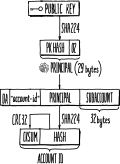
\includegraphics{/images/13-account-id.svg}
\end{figure}

This design decision offers several benefits:
\begin{itemize}
  \item
    Account identifiers occupy about 50\% less memory than \code{(principal, subaccount)} tuples, enabling the ICP ledger to fit a larger account book in memory.
  \item
    A uniform 32-byte account structure makes it easy to find a unique and compact textual representation for accounts.
\end{itemize}

The concept of account identifiers also adds a few problems:
\begin{itemize}
  \item
    Account identifiers is yet another concept that people need to understand.
    The \sc{ic} is already heavy on new ideas and terminology; unnecessary complication does not help adoption.
    For example, a few confused developers tried to pass principal bytes as an account identifier.
  \item
    The account identifier is a one-way function of the principal and the subaccount.
    This property makes the ledger less transparent and complicates error recovery.
    For example, if a client uses custom subaccounts but then forgets what they were, this client can lose tokens.
    Another example: one developer used an invalid subaccount during the account identifier computation and lost a few hundred ICP.
    Since the ledger sees hashed data, it cannot validate the inputs.
  \item
    The opaqueness of identifiers limits the types of applications and payment flows developers can build on top of the ledger.
    For example, if the payer uses custom subaccounts, a canister cannot inspect ledger blocks and easily detect incoming transactions.
\end{itemize}

\section{transactions-and-blocks}{Transactions and blocks}

The \href{https://rosetta-api.org}{Rosetta API} expects a blockchain to have \em{blocks} containing \em{transactions}.
Smart contracts on the IC do not have access to raw blocks and messages within them, so the ICP ledger models its own ``blockchain'' to satisfy the Rosetta data model. 
Each ledger operation, such as minting or transferring tokens, becomes a transaction that the ledger wraps into a unique block and adds to the chain.

\begin{figure}[grayscale-diagram]
\marginnote{mn-blocks}{
  The structure of a block in the ICP ledger.
  Each block contains one transaction and the previous block's hash for the chain validation.
}
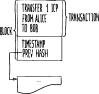
\includegraphics{/images/13-blocks.svg}
\end{figure}

The ICP ledger uses \href{https://developers.google.com/protocol-buffers}{Protocol Buffers} to encode transactions and blocks.
This encoding offers a few benefits:
\begin{itemize}
  \item
    Protocol Buffers offer solid tooling (including a \href{https://docs.buf.build/breaking/overview}{breaking change detector}) that allowed the team to launch the ledger quicker.
  \item
    The \href{https://developers.google.com/protocol-buffers/docs/encoding}{encoding} is simple and easy to implement in a memory-constrained device, such as a \href{https://www.ledger.com/}{Ledger} hardware wallet.
  \item
    The encoding is compact and efficient, comparable to the custom \href{https://developer.bitcoin.org/reference/transactions.html#raw-transaction-format}{Bitcoin serialization format}.
\end{itemize}

The main disadvantage of the Protocol Buffers encoding is its \href{https://developers.google.com/protocol-buffers/docs/encoding#implications}{non-determinism}.
If you start from a block, decode it into a data structure, and encode it according to the \href{https://github.com/dfinity/ic/blob/5248f11c18ca564881bbb82a4eb6915efb7ca62f/rs/rosetta-api/icp_ledger/proto/ic_ledger/pb/v1/types.proto}{Protocol Buffer scheme}, you might end up with bytes that differ from the original.

The ICP ledger uses a deterministic Protocol Buffer encoder to mitigate the non-determinism issue.
The ICP ledger specification describes the \href{https://internetcomputer.org/docs/current/references/ledger/#_chaining_ledger_blocks}{exact encoding} that implementations should use.

\section{validation}{Block validation}

Clients talking to the ledger from outside the IC, such as Rosetta nodes, need to validate that the transaction data they receive from the internet is trustworthy.
Bitcoin blocks are inherently expensive to fake because they rely on a \href{https://en.wikipedia.org/wiki/Proof_of_work}{proof-of-work} mechanism.
The ICP ledger, on the other hand, depends on chain-key cryptography for block validation.

The only way to validate a block with a specific index is to request this block from the ledger using an update call.
Such a request usually takes only a few seconds, but requesting a certificate for each block is impractical: fetching a million blocks individually at the one-block-per-second rate would take about twelve days.

Luckily, we need the IC signatures to validate only the latest block; we can follow the parent hash links starting from the oldest block to authenticate the rest.
This approach enables us to fetch most of the chain using fast queries, reducing the synching time of a million blocks to a few minutes.

\begin{figure}[grayscale-diagram]
  \marginnote{mn-block-validation}{
    The validation scheme for the ICP block synchronization protocol.
    The validator fetches a certificate for the tip of the chain and follows the hash links to validate older blocks.
  }
  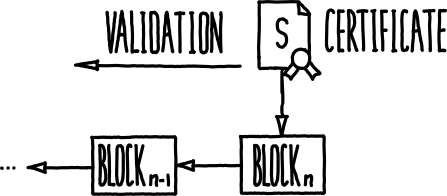
\includegraphics{/images/13-validation.svg}
\end{figure}

The \href{https://medium.com/dfinity/how-internet-computer-responses-are-certified-as-authentic-2ff1bb1ea659}{certified variables} feature of the IC enables another minor optimization.
Each time the ledger records a new \href{#transactions-and-blocks}{block}, it writes the block hash to the \href{https://internetcomputer.org/docs/current/references/ic-interface-spec#state-tree-certified-data}{certified data} section.
With this optimization, the caller can also use a query call to obtain the initial certificate.

\section{tx-dedup}{Transaction deduplication}

The IC has a mechanism protecting against message replay attacks.
Each ingress message has an explicit \href{https://internetcomputer.org/docs/current/references/ic-interface-spec/#authentication}{expiry time}; the IC guarantees to remember accepted messages until they expire.
The allowed expiry window is only a few minutes for scalability reasons: the larger the expiry window, the more messages the IC must remember to prevent replay attacks.

The limited message expiry creates an issue for applications not hosted on the IC.
If a ledger client attempted to transfer funds and then lost network connectivity for a few minutes, there might be no way of checking the outcome of the transfer.
Re-sending the original message with the same timestamp and nonce might not work because the IC time might have moved beyond the expiry window.
Re-sending a new message with the same payload but a different nonce and expiry time might result in executing the same transfer twice.

The ICP ledger addresses the idempotency problem by introducing another layer of transaction deduplication.
The ledger remembers all transactions that happened in the last 24 hours.
If it receives another transfer with precisely the same arguments, it returns an error indicating that the transaction is a duplicate.

This deduplication mechanism is also helpful for companies offering \href{https://www.coindesk.com/learn/what-is-crypto-custody/}{custody services}, such as \href{https://www.coinbase.com}{Coinbase} and \href{https://www.sygnum.com}{Syngnum}.
These companies hold the private key controlling your assets in a safe place in exchange for a fee.
Signing messages with that key is an expensive and slow operation.
Without the deduplication mechanism, the system executing an ICP transfer would have only a few minutes to send and confirm the transaction.
The ledger-level deduplication allows such systems to pre-sign many messages with identical arguments but different expiry windows without the risk of applying the same transaction twice.

\section{storage-and-archives}{Storage and archives}

At the time of the initial ICP ledger design, the available canister memory was scarce.
Canisters could use up to four gigabytes of main memory and up to four gigabytes of stable memory for code upgrades.
There needed to be more than the capacity of a single canister to store an entire transaction history.

The team solved the storage issue beautifully.
When the transaction history grows above a pre-configured threshold, the ledger creates a new canister, an \em{archive node}, and moves old transactions to the archive memory.
The ledger spawns a new archive node when the previous archive node becomes full.

\begin{figure}[grayscale-diagram]
  \marginnote{mn-archives}{
    The ICP ledger delegates the storage of past transactions to archive canisters, reserving its memory for data structures required to validate new transactions.
  }
  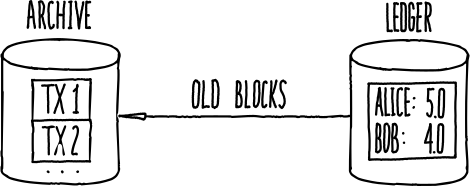
\includegraphics{/images/13-archives.svg}
\end{figure}

With the archive nodes taking care of the transaction history, the ICP ledger needs to store only a few data structures required to validate new transactions, such as the latest account balances and recent transactions.

As of December 2022, the ICP ledger stores account balances in the main memory limited to a few gigabytes.
If the balance map size ever approaches the limit, the ICP ledger will \href{https://github.com/dfinity/ic/blob/a26b66d0bf5dea702e20da7218ceb6a5ee16fbbb/rs/rosetta-api/ledger_canister_core/src/ledger.rs#L192-L213}{burn tokens} on accounts with the smallest balances to free up space for new transactions.
Burning tokens is not as scary as it sounds:
\begin{itemize}
  \item
    As of December 2022, the ICP ledger uses only a few percent of the available capacity, so there is plenty of room to grow.
  \item
    Many accounts hold ``dust'' the owners cannot spend.
    The ledger will trim such accounts in the first place.
  \item
    The transaction log reflects these burns; affected users can ask for a reimbursement.
\end{itemize}

The team plans to move the balance map to the stable memory storage, significantly increasing the size limit.

\section{tx-sigs}{Transaction signatures}

The ICP ledger relies on the IC for signature validation and does not retain signatures in the transaction history.
There are several reasons for this design decision:
\begin{enumerate}
  \item
    As of December 2022, canisters on the IC cannot access ingress message \href{https://internetcomputer.org/docs/current/references/ic-interface-spec#signatures}{signatures}.
  \item
    Inter-canister messages on the same subnet bear no signatures because they reside in the same trust domain.
  \item
    Cross-subnet messages bear signatures\sidenote{sn-message-signatures}{
        The truth is slightly more complicated: the \href{/posts/08-ic-xnet.html}{XNet protocol} contains signatures for message batches, also known as \href{/posts/08-ic-xnet.html#stream-certification}{streams}.
        Validating individual messages requires merkle tree manipulation.
    }, but canisters have no access to them.
\end{enumerate}

Due to these obstacles, the transaction signatures are ephemeral: they exist in the IC blocks at the base layer of the protocol but not in the ICP ledger history.

Even though a few significant changes to the base protocol could resolve the technical issues, retaining transaction witnesses at the ICP ledger layer would have a downside: the space required to store these witnesses would exceed the transaction data by an order of magnitude (most transactions are tiny, about one hundred bytes).

This design reminds me of Bitcoin's \href{https://en.wikipedia.org/wiki/SegWit}{Segregated Witnesses} (\em{SegWit}) proposal separating the transaction data from unlock scripts.
SegWit transactions require signatures for validation, but \href{https://en.bitcoinwiki.org/wiki/Simplified_Payment_Verification}{Simple Payment Verification} nodes get blocks without signatures to save storage space and bandwidth.

\section{references}{References}
\begin{itemize}
  \item
    The \href{https://github.com/dfinity/ic/tree/59ad371332f26ee1af54a15c568dd10a2093224c/rs/rosetta-api/icp_ledger/ledger}{ICP ledger implementation} in Rust.
    This code moves your ICP tokens on the IC.
  \item
    The official developer documentation for the \href{https://internetcomputer.org/docs/current/developer-docs/integrations/ledger/}{ICP ledger} and the \href{https://internetcomputer.org/docs/current/developer-docs/integrations/rosetta/}{Rosetta node}.
  \item
    The ICP ledger \href{https://internetcomputer.org/docs/current/references/ledger}{specification}.
  \item
    The \href{https://github.com/dfinity/ledger-ref}{reference implementation} of the ICP ledger in Motoko.
    This implementation is a model not intended for production, but it can help understand the big picture.
\end{itemize}
\end{document}
